\documentclass[1p]{elsarticle_modified}
%\bibliographystyle{elsarticle-num}

%\usepackage[colorlinks]{hyperref}
%\usepackage{abbrmath_seonhwa} %\Abb, \Ascr, \Acal ,\Abf, \Afrak
\usepackage{amsfonts}
\usepackage{amssymb}
\usepackage{amsmath}
\usepackage{amsthm}
\usepackage{scalefnt}
\usepackage{amsbsy}
\usepackage{kotex}
\usepackage{caption}
\usepackage{subfig}
\usepackage{color}
\usepackage{graphicx}
\usepackage{xcolor} %% white, black, red, green, blue, cyan, magenta, yellow
\usepackage{float}
\usepackage{setspace}
\usepackage{hyperref}

\usepackage{tikz}
\usetikzlibrary{arrows}

\usepackage{multirow}
\usepackage{array} % fixed length table
\usepackage{hhline}

%%%%%%%%%%%%%%%%%%%%%
\makeatletter
\renewcommand*\env@matrix[1][\arraystretch]{%
	\edef\arraystretch{#1}%
	\hskip -\arraycolsep
	\let\@ifnextchar\new@ifnextchar
	\array{*\c@MaxMatrixCols c}}
\makeatother %https://tex.stackexchange.com/questions/14071/how-can-i-increase-the-line-spacing-in-a-matrix
%%%%%%%%%%%%%%%

\usepackage[normalem]{ulem}

\newcommand{\msout}[1]{\ifmmode\text{\sout{\ensuremath{#1}}}\else\sout{#1}\fi}
%SOURCE: \msout is \stkout macro in https://tex.stackexchange.com/questions/20609/strikeout-in-math-mode

\newcommand{\cancel}[1]{
	\ifmmode
	{\color{red}\msout{#1}}
	\else
	{\color{red}\sout{#1}}
	\fi
}

\newcommand{\add}[1]{
	{\color{blue}\uwave{#1}}
}

\newcommand{\replace}[2]{
	\ifmmode
	{\color{red}\msout{#1}}{\color{blue}\uwave{#2}}
	\else
	{\color{red}\sout{#1}}{\color{blue}\uwave{#2}}
	\fi
}

\newcommand{\Sol}{\mathcal{S}} %segment
\newcommand{\D}{D} %diagram
\newcommand{\A}{\mathcal{A}} %arc


%%%%%%%%%%%%%%%%%%%%%%%%%%%%%5 test

\def\sl{\operatorname{\textup{SL}}(2,\Cbb)}
\def\psl{\operatorname{\textup{PSL}}(2,\Cbb)}
\def\quan{\mkern 1mu \triangleright \mkern 1mu}

\theoremstyle{definition}
\newtheorem{thm}{Theorem}[section]
\newtheorem{prop}[thm]{Proposition}
\newtheorem{lem}[thm]{Lemma}
\newtheorem{ques}[thm]{Question}
\newtheorem{cor}[thm]{Corollary}
\newtheorem{defn}[thm]{Definition}
\newtheorem{exam}[thm]{Example}
\newtheorem{rmk}[thm]{Remark}
\newtheorem{alg}[thm]{Algorithm}

\newcommand{\I}{\sqrt{-1}}
\begin{document}

%\begin{frontmatter}
%
%\title{Boundary parabolic representations of knots up to 8 crossings}
%
%%% Group authors per affiliation:
%\author{Yunhi Cho} 
%\address{Department of Mathematics, University of Seoul, Seoul, Korea}
%\ead{yhcho@uos.ac.kr}
%
%
%\author{Seonhwa Kim} %\fnref{s_kim}}
%\address{Center for Geometry and Physics, Institute for Basic Science, Pohang, 37673, Korea}
%\ead{ryeona17@ibs.re.kr}
%
%\author{Hyuk Kim}
%\address{Department of Mathematical Sciences, Seoul National University, Seoul 08826, Korea}
%\ead{hyukkim@snu.ac.kr}
%
%\author{Seokbeom Yoon}
%\address{Department of Mathematical Sciences, Seoul National University, Seoul, 08826,  Korea}
%\ead{sbyoon15@snu.ac.kr}
%
%\begin{abstract}
%We find all boundary parabolic representation of knots up to 8 crossings.
%
%\end{abstract}
%\begin{keyword}
%    \MSC[2010] 57M25 
%\end{keyword}
%
%\end{frontmatter}

%\linenumbers
%\tableofcontents
%
\newcommand\colored[1]{\textcolor{white}{\rule[-0.35ex]{0.8em}{1.4ex}}\kern-0.8em\color{red} #1}%
%\newcommand\colored[1]{\textcolor{white}{ #1}\kern-2.17ex	\textcolor{white}{ #1}\kern-1.81ex	\textcolor{white}{ #1}\kern-2.15ex\color{red}#1	}

{\Large $\underline{11a_{15}~(K11a_{15})}$}

\setlength{\tabcolsep}{10pt}
\renewcommand{\arraystretch}{1.6}
\vspace{1cm}\begin{tabular}{m{100pt}>{\centering\arraybackslash}m{274pt}}
\multirow{5}{120pt}{
	\centering
	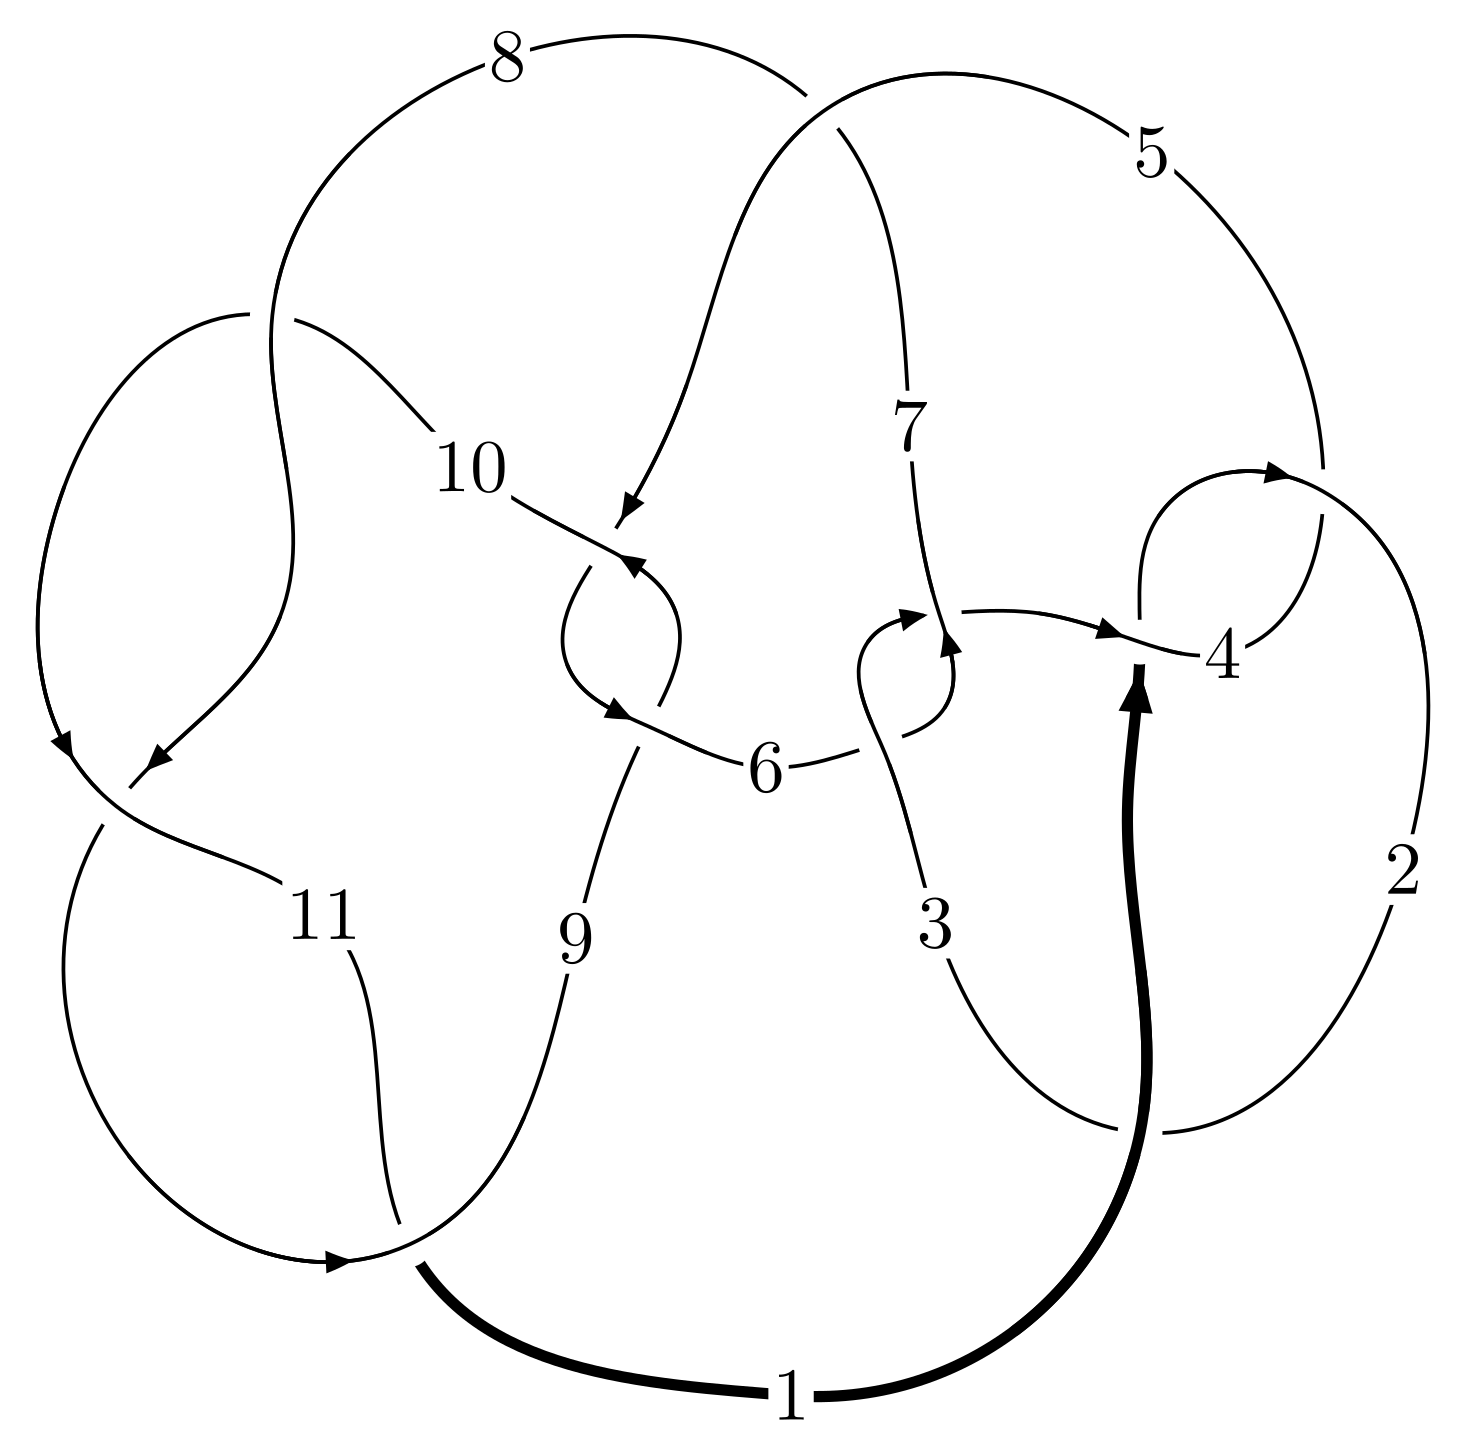
\includegraphics[width=112pt]{../../../GIT/diagram.site/Diagrams/png/264_11a_15.png}\\
\ \ \ A knot diagram\footnotemark}&
\allowdisplaybreaks
\textbf{Linearized knot diagam} \\
\cline{2-2}
 &
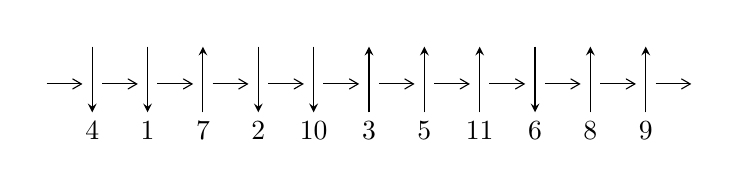
\begin{tikzpicture}[x=20pt, y=17pt]
	% nodes
	\node (C0) at (0, 0) {};
	\node (C1) at (1, 0) {};
	\node (C1U) at (1, +1) {};
	\node (C1D) at (1, -1) {4};

	\node (C2) at (2, 0) {};
	\node (C2U) at (2, +1) {};
	\node (C2D) at (2, -1) {1};

	\node (C3) at (3, 0) {};
	\node (C3U) at (3, +1) {};
	\node (C3D) at (3, -1) {7};

	\node (C4) at (4, 0) {};
	\node (C4U) at (4, +1) {};
	\node (C4D) at (4, -1) {2};

	\node (C5) at (5, 0) {};
	\node (C5U) at (5, +1) {};
	\node (C5D) at (5, -1) {10};

	\node (C6) at (6, 0) {};
	\node (C6U) at (6, +1) {};
	\node (C6D) at (6, -1) {3};

	\node (C7) at (7, 0) {};
	\node (C7U) at (7, +1) {};
	\node (C7D) at (7, -1) {5};

	\node (C8) at (8, 0) {};
	\node (C8U) at (8, +1) {};
	\node (C8D) at (8, -1) {11};

	\node (C9) at (9, 0) {};
	\node (C9U) at (9, +1) {};
	\node (C9D) at (9, -1) {6};

	\node (C10) at (10, 0) {};
	\node (C10U) at (10, +1) {};
	\node (C10D) at (10, -1) {8};

	\node (C11) at (11, 0) {};
	\node (C11U) at (11, +1) {};
	\node (C11D) at (11, -1) {9};
	\node (C12) at (12, 0) {};

	% arrows
	\draw[->,>={angle 60}]
	(C0) edge (C1) (C1) edge (C2) (C2) edge (C3) (C3) edge (C4) (C4) edge (C5) (C5) edge (C6) (C6) edge (C7) (C7) edge (C8) (C8) edge (C9) (C9) edge (C10) (C10) edge (C11) (C11) edge (C12) ;	\draw[->,>=stealth]
	(C1U) edge (C1D) (C2U) edge (C2D) (C3D) edge (C3U) (C4U) edge (C4D) (C5U) edge (C5D) (C6D) edge (C6U) (C7D) edge (C7U) (C8D) edge (C8U) (C9U) edge (C9D) (C10D) edge (C10U) (C11D) edge (C11U) ;
	\end{tikzpicture} \\
\hhline{~~} \\& 
\textbf{Solving Sequence} \\ \cline{2-2} 
 &
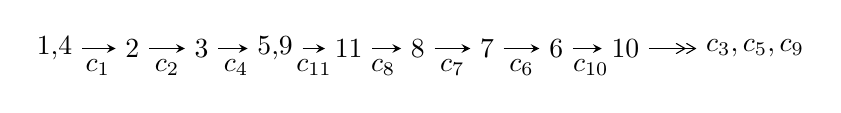
\begin{tikzpicture}[x=25pt, y=7pt]
	% node
	\node (A0) at (-1/8, 0) {1,4};
	\node (A1) at (1, 0) {2};
	\node (A2) at (2, 0) {3};
	\node (A3) at (49/16, 0) {5,9};
	\node (A4) at (33/8, 0) {11};
	\node (A5) at (41/8, 0) {8};
	\node (A6) at (49/8, 0) {7};
	\node (A7) at (57/8, 0) {6};
	\node (A8) at (65/8, 0) {10};
	\node (C1) at (1/2, -1) {$c_{1}$};
	\node (C2) at (3/2, -1) {$c_{2}$};
	\node (C3) at (5/2, -1) {$c_{4}$};
	\node (C4) at (29/8, -1) {$c_{11}$};
	\node (C5) at (37/8, -1) {$c_{8}$};
	\node (C6) at (45/8, -1) {$c_{7}$};
	\node (C7) at (53/8, -1) {$c_{6}$};
	\node (C8) at (61/8, -1) {$c_{10}$};
	\node (A9) at (10, 0) {$c_{3},c_{5},c_{9}$};

	% edge
	\draw[->,>=stealth]	
	(A0) edge (A1) (A1) edge (A2) (A2) edge (A3) (A3) edge (A4) (A4) edge (A5) (A5) edge (A6) (A6) edge (A7) (A7) edge (A8) ;
	\draw[->>,>={angle 60}]	
	(A8) edge (A9);
\end{tikzpicture} \\ 

\end{tabular} \\

\footnotetext{
The image of knot diagram is generated by the software ``\textbf{Draw programme}" developed by Andrew Bartholomew(\url{http://www.layer8.co.uk/maths/draw/index.htm\#Running-draw}), where we modified some parts for our purpose(\url{https://github.com/CATsTAILs/LinksPainter}).
}\phantom \\ \newline 
\centering \textbf{Ideals for irreducible components\footnotemark of $X_{\text{par}}$} 
 
\begin{align*}
I^u_{1}&=\langle 
-1.04308\times10^{20} u^{63}-7.59004\times10^{20} u^{62}+\cdots+3.96371\times10^{19} b+2.83284\times10^{20},\\
\phantom{I^u_{1}}&\phantom{= \langle  }-7.35239\times10^{20} u^{63}-3.87644\times10^{21} u^{62}+\cdots+7.92742\times10^{19} a+5.92603\times10^{20},\\
\phantom{I^u_{1}}&\phantom{= \langle  }u^{64}+7 u^{63}+\cdots-13 u-1\rangle \\
I^u_{2}&=\langle 
b-1,\;u^4+u^3+a- u,\;u^6+u^5- u^4-2 u^3+u+1\rangle \\
I^u_{3}&=\langle 
a^3+b+1,\;a^5+a^4+a^3+2 a^2+a+1,\;u-1\rangle \\
\\
\end{align*}
\raggedright * 3 irreducible components of $\dim_{\mathbb{C}}=0$, with total 75 representations.\\
\footnotetext{All coefficients of polynomials are rational numbers. But the coefficients are sometimes approximated in decimal forms when there is not enough margin.}
\newpage
\renewcommand{\arraystretch}{1}
\centering \section*{I. $I^u_{1}= \langle -1.04\times10^{20} u^{63}-7.59\times10^{20} u^{62}+\cdots+3.96\times10^{19} b+2.83\times10^{20},\;-7.35\times10^{20} u^{63}-3.88\times10^{21} u^{62}+\cdots+7.93\times10^{19} a+5.93\times10^{20},\;u^{64}+7 u^{63}+\cdots-13 u-1 \rangle$}
\flushleft \textbf{(i) Arc colorings}\\
\begin{tabular}{m{7pt} m{180pt} m{7pt} m{180pt} }
\flushright $a_{1}=$&$\begin{pmatrix}1\\0\end{pmatrix}$ \\
\flushright $a_{4}=$&$\begin{pmatrix}0\\u\end{pmatrix}$ \\
\flushright $a_{2}=$&$\begin{pmatrix}1\\u^2\end{pmatrix}$ \\
\flushright $a_{3}=$&$\begin{pmatrix}- u^2+1\\u^2\end{pmatrix}$ \\
\flushright $a_{5}=$&$\begin{pmatrix}- u\\- u^3+u\end{pmatrix}$ \\
\flushright $a_{9}=$&$\begin{pmatrix}9.27463 u^{63}+48.8992 u^{62}+\cdots-37.0886 u-7.47536\\2.63156 u^{63}+19.1488 u^{62}+\cdots-70.8971 u-7.14695\end{pmatrix}$ \\
\flushright $a_{11}=$&$\begin{pmatrix}-5.65805 u^{63}-29.1771 u^{62}+\cdots+32.6675 u+8.99552\\2.08876 u^{63}+9.72032 u^{62}+\cdots+23.9118 u+3.59970\end{pmatrix}$ \\
\flushright $a_{8}=$&$\begin{pmatrix}4.89840 u^{63}+26.5797 u^{62}+\cdots+14.3202 u+4.18773\\4.18435 u^{63}+30.2617 u^{62}+\cdots-83.2794 u-6.53051\end{pmatrix}$ \\
\flushright $a_{7}=$&$\begin{pmatrix}2.16346 u^{63}+8.50706 u^{62}+\cdots+60.6164 u+7.93271\\7.04006 u^{63}+48.8776 u^{62}+\cdots-118.375 u-9.20353\end{pmatrix}$ \\
\flushright $a_{6}=$&$\begin{pmatrix}-1.17863 u^{63}-5.74060 u^{62}+\cdots+14.7171 u+3.28124\\3.74498 u^{63}+23.4799 u^{62}+\cdots-36.4181 u-2.38859\end{pmatrix}$ \\
\flushright $a_{10}=$&$\begin{pmatrix}-18.2987 u^{63}-107.518 u^{62}+\cdots+156.183 u+15.9335\\-6.10504 u^{63}-50.2563 u^{62}+\cdots+221.478 u+19.9762\end{pmatrix}$\\ \flushright $a_{10}=$&$\begin{pmatrix}-18.2987 u^{63}-107.518 u^{62}+\cdots+156.183 u+15.9335\\-6.10504 u^{63}-50.2563 u^{62}+\cdots+221.478 u+19.9762\end{pmatrix}$\\&\end{tabular}
\flushleft \textbf{(ii) Obstruction class $= -1$}\\~\\
\flushleft \textbf{(iii) Cusp Shapes $= \frac{154506605926350535629}{9909273683398550218} u^{63}+\frac{2873546855263844556609}{39637094733594200872} u^{62}+\cdots+\frac{3763600436801685598541}{39637094733594200872} u+\frac{551008705357518405765}{39637094733594200872}$}\\~\\
\newpage\renewcommand{\arraystretch}{1}
\flushleft \textbf{(iv) u-Polynomials at the component}\newline \\
\begin{tabular}{m{50pt}|m{274pt}}
Crossings & \hspace{64pt}u-Polynomials at each crossing \\
\hline $$\begin{aligned}c_{1},c_{4}\end{aligned}$$&$\begin{aligned}
&u^{64}-7 u^{63}+\cdots+13 u-1
\end{aligned}$\\
\hline $$\begin{aligned}c_{2}\end{aligned}$$&$\begin{aligned}
&u^{64}+29 u^{63}+\cdots+37 u+1
\end{aligned}$\\
\hline $$\begin{aligned}c_{3},c_{6}\end{aligned}$$&$\begin{aligned}
&u^{64}-2 u^{63}+\cdots-128 u+32
\end{aligned}$\\
\hline $$\begin{aligned}c_{5},c_{9}\end{aligned}$$&$\begin{aligned}
&u^{64}+2 u^{63}+\cdots+128 u-64
\end{aligned}$\\
\hline $$\begin{aligned}c_{7}\end{aligned}$$&$\begin{aligned}
&u^{64}+3 u^{63}+\cdots-2001 u-1609
\end{aligned}$\\
\hline $$\begin{aligned}c_{8},c_{10},c_{11}\end{aligned}$$&$\begin{aligned}
&u^{64}+8 u^{63}+\cdots+4 u+1
\end{aligned}$\\
\hline
\end{tabular}\\~\\
\newpage\renewcommand{\arraystretch}{1}
\flushleft \textbf{(v) Riley Polynomials at the component}\newline \\
\begin{tabular}{m{50pt}|m{274pt}}
Crossings & \hspace{64pt}Riley Polynomials at each crossing \\
\hline $$\begin{aligned}c_{1},c_{4}\end{aligned}$$&$\begin{aligned}
&y^{64}-29 y^{63}+\cdots-37 y+1
\end{aligned}$\\
\hline $$\begin{aligned}c_{2}\end{aligned}$$&$\begin{aligned}
&y^{64}+19 y^{63}+\cdots-3653 y+1
\end{aligned}$\\
\hline $$\begin{aligned}c_{3},c_{6}\end{aligned}$$&$\begin{aligned}
&y^{64}-36 y^{63}+\cdots-20992 y+1024
\end{aligned}$\\
\hline $$\begin{aligned}c_{5},c_{9}\end{aligned}$$&$\begin{aligned}
&y^{64}+42 y^{63}+\cdots+24576 y+4096
\end{aligned}$\\
\hline $$\begin{aligned}c_{7}\end{aligned}$$&$\begin{aligned}
&y^{64}-37 y^{63}+\cdots+70611765 y+2588881
\end{aligned}$\\
\hline $$\begin{aligned}c_{8},c_{10},c_{11}\end{aligned}$$&$\begin{aligned}
&y^{64}-64 y^{63}+\cdots+20 y+1
\end{aligned}$\\
\hline
\end{tabular}\\~\\
\newpage\flushleft \textbf{(vi) Complex Volumes and Cusp Shapes}
$$\begin{array}{c|c|c}  
\text{Solutions to }I^u_{1}& \I (\text{vol} + \sqrt{-1}CS) & \text{Cusp shape}\\
 \hline 
\begin{aligned}
u &= \phantom{-}0.851015 + 0.553122 I \\
a &= \phantom{-}3.09153 + 1.65651 I \\
b &= -1.403090 + 0.050018 I\end{aligned}
 & \phantom{-}3.26372 - 2.22000 I & \phantom{-0.000000 } 0 \\ \hline\begin{aligned}
u &= \phantom{-}0.851015 - 0.553122 I \\
a &= \phantom{-}3.09153 - 1.65651 I \\
b &= -1.403090 - 0.050018 I\end{aligned}
 & \phantom{-}3.26372 + 2.22000 I & \phantom{-0.000000 } 0 \\ \hline\begin{aligned}
u &= -0.468773 + 0.906872 I \\
a &= \phantom{-}0.474383 - 0.050538 I \\
b &= -0.493081 + 0.851380 I\end{aligned}
 & \phantom{-}5.97499 - 4.90532 I & \phantom{-0.000000 } 0 \\ \hline\begin{aligned}
u &= -0.468773 - 0.906872 I \\
a &= \phantom{-}0.474383 + 0.050538 I \\
b &= -0.493081 - 0.851380 I\end{aligned}
 & \phantom{-}5.97499 + 4.90532 I & \phantom{-0.000000 } 0 \\ \hline\begin{aligned}
u &= \phantom{-}0.957619 + 0.369938 I \\
a &= -1.152950 - 0.390386 I \\
b &= \phantom{-}0.170773 - 0.218203 I\end{aligned}
 & -1.81999 - 1.29187 I & \phantom{-0.000000 } 0 \\ \hline\begin{aligned}
u &= \phantom{-}0.957619 - 0.369938 I \\
a &= -1.152950 + 0.390386 I \\
b &= \phantom{-}0.170773 + 0.218203 I\end{aligned}
 & -1.81999 + 1.29187 I & \phantom{-0.000000 } 0 \\ \hline\begin{aligned}
u &= -0.554715 + 0.872769 I \\
a &= \phantom{-}0.811122 - 0.142635 I \\
b &= -0.681254 - 0.756164 I\end{aligned}
 & \phantom{-}6.56660 + 0.51971 I & \phantom{-0.000000 } 0 \\ \hline\begin{aligned}
u &= -0.554715 - 0.872769 I \\
a &= \phantom{-}0.811122 + 0.142635 I \\
b &= -0.681254 + 0.756164 I\end{aligned}
 & \phantom{-}6.56660 - 0.51971 I & \phantom{-0.000000 } 0 \\ \hline\begin{aligned}
u &= -0.513391 + 0.900925 I \\
a &= \phantom{-}2.49041 + 0.02335 I \\
b &= -1.46519 + 0.07102 I\end{aligned}
 & \phantom{-}8.42241 - 2.26761 I & \phantom{-0.000000 } 0 \\ \hline\begin{aligned}
u &= -0.513391 - 0.900925 I \\
a &= \phantom{-}2.49041 - 0.02335 I \\
b &= -1.46519 - 0.07102 I\end{aligned}
 & \phantom{-}8.42241 + 2.26761 I & \phantom{-0.000000 } 0\\
 \hline 
 \end{array}$$\newpage$$\begin{array}{c|c|c}  
\text{Solutions to }I^u_{1}& \I (\text{vol} + \sqrt{-1}CS) & \text{Cusp shape}\\
 \hline 
\begin{aligned}
u &= -0.798906 + 0.537570 I \\
a &= \phantom{-}0.556103 + 0.446579 I \\
b &= -1.208400 + 0.288039 I\end{aligned}
 & \phantom{-}2.82835 + 0.98333 I & \phantom{-}5.99923 - 3.36293 I \\ \hline\begin{aligned}
u &= -0.798906 - 0.537570 I \\
a &= \phantom{-}0.556103 - 0.446579 I \\
b &= -1.208400 - 0.288039 I\end{aligned}
 & \phantom{-}2.82835 - 0.98333 I & \phantom{-}5.99923 + 3.36293 I \\ \hline\begin{aligned}
u &= \phantom{-}0.684326 + 0.663082 I \\
a &= -2.47318 - 0.47845 I \\
b &= \phantom{-}1.52333 + 0.22252 I\end{aligned}
 & \phantom{-}8.25062 + 3.46517 I & \phantom{-}6.83292 + 0. I\phantom{ +0.000000I} \\ \hline\begin{aligned}
u &= \phantom{-}0.684326 - 0.663082 I \\
a &= -2.47318 + 0.47845 I \\
b &= \phantom{-}1.52333 - 0.22252 I\end{aligned}
 & \phantom{-}8.25062 - 3.46517 I & \phantom{-}6.83292 + 0. I\phantom{ +0.000000I} \\ \hline\begin{aligned}
u &= -0.892560 + 0.567255 I \\
a &= \phantom{-}0.55087 - 1.60438 I \\
b &= -1.080850 - 0.394220 I\end{aligned}
 & \phantom{-}2.50515 + 3.47504 I & \phantom{-0.000000 } 0 \\ \hline\begin{aligned}
u &= -0.892560 - 0.567255 I \\
a &= \phantom{-}0.55087 + 1.60438 I \\
b &= -1.080850 + 0.394220 I\end{aligned}
 & \phantom{-}2.50515 - 3.47504 I & \phantom{-0.000000 } 0 \\ \hline\begin{aligned}
u &= -0.426816 + 0.971335 I \\
a &= -1.81629 - 0.41191 I \\
b &= \phantom{-}1.53562 - 0.30377 I\end{aligned}
 & \phantom{-}12.5775 - 9.1285 I & \phantom{-0.000000 } 0 \\ \hline\begin{aligned}
u &= -0.426816 - 0.971335 I \\
a &= -1.81629 + 0.41191 I \\
b &= \phantom{-}1.53562 + 0.30377 I\end{aligned}
 & \phantom{-}12.5775 + 9.1285 I & \phantom{-0.000000 } 0 \\ \hline\begin{aligned}
u &= \phantom{-}0.773933 + 0.525049 I \\
a &= \phantom{-}0.224362 + 0.775639 I \\
b &= -0.586485 - 0.667589 I\end{aligned}
 & \phantom{-}1.392230 + 0.239734 I & \phantom{-}4.64422 + 0. I\phantom{ +0.000000I} \\ \hline\begin{aligned}
u &= \phantom{-}0.773933 - 0.525049 I \\
a &= \phantom{-}0.224362 - 0.775639 I \\
b &= -0.586485 + 0.667589 I\end{aligned}
 & \phantom{-}1.392230 - 0.239734 I & \phantom{-}4.64422 + 0. I\phantom{ +0.000000I}\\
 \hline 
 \end{array}$$\newpage$$\begin{array}{c|c|c}  
\text{Solutions to }I^u_{1}& \I (\text{vol} + \sqrt{-1}CS) & \text{Cusp shape}\\
 \hline 
\begin{aligned}
u &= \phantom{-}0.926326 + 0.128275 I \\
a &= \phantom{-}0.70787 + 3.19878 I \\
b &= -0.967057 + 0.104240 I\end{aligned}
 & \phantom{-}0.047902 - 0.498911 I & \phantom{-}2.1353 - 14.8724 I \\ \hline\begin{aligned}
u &= \phantom{-}0.926326 - 0.128275 I \\
a &= \phantom{-}0.70787 - 3.19878 I \\
b &= -0.967057 - 0.104240 I\end{aligned}
 & \phantom{-}0.047902 + 0.498911 I & \phantom{-}2.1353 + 14.8724 I \\ \hline\begin{aligned}
u &= \phantom{-}0.912042 + 0.554130 I \\
a &= \phantom{-}1.43049 + 0.51144 I \\
b &= -0.469774 + 0.774809 I\end{aligned}
 & \phantom{-}0.93426 - 4.62344 I & \phantom{-0.000000 } 0 \\ \hline\begin{aligned}
u &= \phantom{-}0.912042 - 0.554130 I \\
a &= \phantom{-}1.43049 - 0.51144 I \\
b &= -0.469774 - 0.774809 I\end{aligned}
 & \phantom{-}0.93426 + 4.62344 I & \phantom{-0.000000 } 0 \\ \hline\begin{aligned}
u &= -0.965340 + 0.501059 I \\
a &= -0.068579 - 0.710395 I \\
b &= \phantom{-}0.040956 - 0.606385 I\end{aligned}
 & -1.01229 + 4.28688 I & \phantom{-0.000000 } 0 \\ \hline\begin{aligned}
u &= -0.965340 - 0.501059 I \\
a &= -0.068579 + 0.710395 I \\
b &= \phantom{-}0.040956 + 0.606385 I\end{aligned}
 & -1.01229 - 4.28688 I & \phantom{-0.000000 } 0 \\ \hline\begin{aligned}
u &= -0.796135 + 0.411444 I \\
a &= -0.560743 + 0.887793 I \\
b &= -0.166184 + 0.699479 I\end{aligned}
 & -0.262566 - 0.498963 I & \phantom{-}2.74689 - 0.51399 I \\ \hline\begin{aligned}
u &= -0.796135 - 0.411444 I \\
a &= -0.560743 - 0.887793 I \\
b &= -0.166184 - 0.699479 I\end{aligned}
 & -0.262566 + 0.498963 I & \phantom{-}2.74689 + 0.51399 I \\ \hline\begin{aligned}
u &= \phantom{-}1.090500 + 0.201214 I \\
a &= -0.486035 + 0.573321 I \\
b &= -0.004735 + 0.287127 I\end{aligned}
 & -2.28356 - 0.63564 I & \phantom{-0.000000 } 0 \\ \hline\begin{aligned}
u &= \phantom{-}1.090500 - 0.201214 I \\
a &= -0.486035 - 0.573321 I \\
b &= -0.004735 - 0.287127 I\end{aligned}
 & -2.28356 + 0.63564 I & \phantom{-0.000000 } 0\\
 \hline 
 \end{array}$$\newpage$$\begin{array}{c|c|c}  
\text{Solutions to }I^u_{1}& \I (\text{vol} + \sqrt{-1}CS) & \text{Cusp shape}\\
 \hline 
\begin{aligned}
u &= -0.457914 + 0.741659 I \\
a &= -0.755401 + 0.029158 I \\
b &= \phantom{-}0.358616 - 0.179646 I\end{aligned}
 & \phantom{-}2.38826 - 1.27360 I & \phantom{-}1.00000 + 1.24138 I \\ \hline\begin{aligned}
u &= -0.457914 - 0.741659 I \\
a &= -0.755401 - 0.029158 I \\
b &= \phantom{-}0.358616 + 0.179646 I\end{aligned}
 & \phantom{-}2.38826 + 1.27360 I & \phantom{-}1.00000 - 1.24138 I \\ \hline\begin{aligned}
u &= -0.656679 + 0.923424 I \\
a &= -2.02373 + 0.73995 I \\
b &= \phantom{-}1.58190 + 0.20504 I\end{aligned}
 & \phantom{-}14.1398 + 3.9767 I & \phantom{-0.000000 } 0 \\ \hline\begin{aligned}
u &= -0.656679 - 0.923424 I \\
a &= -2.02373 - 0.73995 I \\
b &= \phantom{-}1.58190 - 0.20504 I\end{aligned}
 & \phantom{-}14.1398 - 3.9767 I & \phantom{-0.000000 } 0 \\ \hline\begin{aligned}
u &= \phantom{-}0.968165 + 0.622296 I \\
a &= -2.05377 - 2.02763 I \\
b &= \phantom{-}1.51383 - 0.27793 I\end{aligned}
 & \phantom{-}7.38800 - 8.47452 I & \phantom{-0.000000 } 0 \\ \hline\begin{aligned}
u &= \phantom{-}0.968165 - 0.622296 I \\
a &= -2.05377 + 2.02763 I \\
b &= \phantom{-}1.51383 + 0.27793 I\end{aligned}
 & \phantom{-}7.38800 + 8.47452 I & \phantom{-0.000000 } 0 \\ \hline\begin{aligned}
u &= -0.814156 + 0.225854 I \\
a &= \phantom{-}0.488791 - 0.388735 I \\
b &= \phantom{-}1.388550 - 0.248297 I\end{aligned}
 & \phantom{-}4.72329 - 3.85111 I & \phantom{-}9.95444 - 1.38614 I \\ \hline\begin{aligned}
u &= -0.814156 - 0.225854 I \\
a &= \phantom{-}0.488791 + 0.388735 I \\
b &= \phantom{-}1.388550 + 0.248297 I\end{aligned}
 & \phantom{-}4.72329 + 3.85111 I & \phantom{-}9.95444 + 1.38614 I \\ \hline\begin{aligned}
u &= -1.102490 + 0.469558 I \\
a &= \phantom{-}0.183729 + 1.038150 I \\
b &= \phantom{-}1.304930 + 0.108429 I\end{aligned}
 & \phantom{-}2.70253 + 6.62281 I & \phantom{-0.000000 } 0 \\ \hline\begin{aligned}
u &= -1.102490 - 0.469558 I \\
a &= \phantom{-}0.183729 - 1.038150 I \\
b &= \phantom{-}1.304930 - 0.108429 I\end{aligned}
 & \phantom{-}2.70253 - 6.62281 I & \phantom{-0.000000 } 0\\
 \hline 
 \end{array}$$\newpage$$\begin{array}{c|c|c}  
\text{Solutions to }I^u_{1}& \I (\text{vol} + \sqrt{-1}CS) & \text{Cusp shape}\\
 \hline 
\begin{aligned}
u &= -1.078950 + 0.604214 I \\
a &= -0.829008 + 0.571399 I \\
b &= \phantom{-}0.382661 + 0.323178 I\end{aligned}
 & \phantom{-}0.55603 + 6.40064 I & \phantom{-0.000000 } 0 \\ \hline\begin{aligned}
u &= -1.078950 - 0.604214 I \\
a &= -0.829008 - 0.571399 I \\
b &= \phantom{-}0.382661 - 0.323178 I\end{aligned}
 & \phantom{-}0.55603 - 6.40064 I & \phantom{-0.000000 } 0 \\ \hline\begin{aligned}
u &= \phantom{-}1.190520 + 0.380856 I \\
a &= \phantom{-}0.168620 - 1.294890 I \\
b &= \phantom{-}1.380510 - 0.021197 I\end{aligned}
 & \phantom{-}2.11698 - 1.35062 I & \phantom{-0.000000 } 0 \\ \hline\begin{aligned}
u &= \phantom{-}1.190520 - 0.380856 I \\
a &= \phantom{-}0.168620 + 1.294890 I \\
b &= \phantom{-}1.380510 + 0.021197 I\end{aligned}
 & \phantom{-}2.11698 + 1.35062 I & \phantom{-0.000000 } 0 \\ \hline\begin{aligned}
u &= \phantom{-}1.27051\phantom{ +0.000000I} \\
a &= \phantom{-}0.853993\phantom{ +0.000000I} \\
b &= -1.36931\phantom{ +0.000000I}\end{aligned}
 & \phantom{-}1.81885\phantom{ +0.000000I} & \phantom{-0.000000 } 0 \\ \hline\begin{aligned}
u &= \phantom{-}1.269650 + 0.066401 I \\
a &= -0.275750 - 1.025770 I \\
b &= -0.479663 - 0.698680 I\end{aligned}
 & -0.29295 + 2.27028 I & \phantom{-0.000000 } 0 \\ \hline\begin{aligned}
u &= \phantom{-}1.269650 - 0.066401 I \\
a &= -0.275750 + 1.025770 I \\
b &= -0.479663 + 0.698680 I\end{aligned}
 & -0.29295 - 2.27028 I & \phantom{-0.000000 } 0 \\ \hline\begin{aligned}
u &= -1.078140 + 0.686845 I \\
a &= -0.219031 - 0.278038 I \\
b &= -0.763986 + 0.723012 I\end{aligned}
 & \phantom{-}4.97472 + 5.25194 I & \phantom{-0.000000 } 0 \\ \hline\begin{aligned}
u &= -1.078140 - 0.686845 I \\
a &= -0.219031 + 0.278038 I \\
b &= -0.763986 - 0.723012 I\end{aligned}
 & \phantom{-}4.97472 - 5.25194 I & \phantom{-0.000000 } 0 \\ \hline\begin{aligned}
u &= -1.037310 + 0.770242 I \\
a &= -1.42167 + 0.83458 I \\
b &= \phantom{-}1.59003 - 0.15683 I\end{aligned}
 & \phantom{-}12.97910 + 2.20987 I & \phantom{-0.000000 } 0\\
 \hline 
 \end{array}$$\newpage$$\begin{array}{c|c|c}  
\text{Solutions to }I^u_{1}& \I (\text{vol} + \sqrt{-1}CS) & \text{Cusp shape}\\
 \hline 
\begin{aligned}
u &= -1.037310 - 0.770242 I \\
a &= -1.42167 - 0.83458 I \\
b &= \phantom{-}1.59003 + 0.15683 I\end{aligned}
 & \phantom{-}12.97910 - 2.20987 I & \phantom{-0.000000 } 0 \\ \hline\begin{aligned}
u &= \phantom{-}0.016268 + 0.696606 I \\
a &= -1.34669 + 0.52337 I \\
b &= \phantom{-}1.41254 - 0.07728 I\end{aligned}
 & \phantom{-}5.65313 - 2.65309 I & \phantom{-}8.42225 + 3.34216 I \\ \hline\begin{aligned}
u &= \phantom{-}0.016268 - 0.696606 I \\
a &= -1.34669 - 0.52337 I \\
b &= \phantom{-}1.41254 + 0.07728 I\end{aligned}
 & \phantom{-}5.65313 + 2.65309 I & \phantom{-}8.42225 - 3.34216 I \\ \hline\begin{aligned}
u &= -1.109430 + 0.686273 I \\
a &= \phantom{-}1.83349 - 1.64073 I \\
b &= -1.46331 - 0.12160 I\end{aligned}
 & \phantom{-}6.60913 + 8.11292 I & \phantom{-0.000000 } 0 \\ \hline\begin{aligned}
u &= -1.109430 - 0.686273 I \\
a &= \phantom{-}1.83349 + 1.64073 I \\
b &= -1.46331 + 0.12160 I\end{aligned}
 & \phantom{-}6.60913 - 8.11292 I & \phantom{-0.000000 } 0 \\ \hline\begin{aligned}
u &= -1.131050 + 0.671760 I \\
a &= \phantom{-}1.043840 - 0.815468 I \\
b &= -0.438312 - 0.882770 I\end{aligned}
 & \phantom{-}3.96365 + 10.71220 I & \phantom{-0.000000 } 0 \\ \hline\begin{aligned}
u &= -1.131050 - 0.671760 I \\
a &= \phantom{-}1.043840 + 0.815468 I \\
b &= -0.438312 + 0.882770 I\end{aligned}
 & \phantom{-}3.96365 - 10.71220 I & \phantom{-0.000000 } 0 \\ \hline\begin{aligned}
u &= -1.172420 + 0.678120 I \\
a &= -1.26144 + 1.95035 I \\
b &= \phantom{-}1.51825 + 0.32917 I\end{aligned}
 & \phantom{-}10.2926 + 15.1288 I & \phantom{-0.000000 } 0 \\ \hline\begin{aligned}
u &= -1.172420 - 0.678120 I \\
a &= -1.26144 - 1.95035 I \\
b &= \phantom{-}1.51825 - 0.32917 I\end{aligned}
 & \phantom{-}10.2926 - 15.1288 I & \phantom{-0.000000 } 0 \\ \hline\begin{aligned}
u &= \phantom{-}1.350730 + 0.109045 I \\
a &= -0.034825 + 0.580788 I \\
b &= \phantom{-}1.50631 + 0.25249 I\end{aligned}
 & \phantom{-}6.16621 + 5.77451 I & \phantom{-0.000000 } 0\\
 \hline 
 \end{array}$$\newpage$$\begin{array}{c|c|c}  
\text{Solutions to }I^u_{1}& \I (\text{vol} + \sqrt{-1}CS) & \text{Cusp shape}\\
 \hline 
\begin{aligned}
u &= \phantom{-}1.350730 - 0.109045 I \\
a &= -0.034825 - 0.580788 I \\
b &= \phantom{-}1.50631 - 0.25249 I\end{aligned}
 & \phantom{-}6.16621 - 5.77451 I & \phantom{-0.000000 } 0 \\ \hline\begin{aligned}
u &= -0.004404 + 0.249946 I \\
a &= -1.65033 - 0.59592 I \\
b &= -0.278953 + 0.383140 I\end{aligned}
 & \phantom{-}0.309124 - 1.130770 I & \phantom{-}3.85993 + 6.08046 I \\ \hline\begin{aligned}
u &= -0.004404 - 0.249946 I \\
a &= -1.65033 + 0.59592 I \\
b &= -0.278953 - 0.383140 I\end{aligned}
 & \phantom{-}0.309124 + 1.130770 I & \phantom{-}3.85993 - 6.08046 I \\ \hline\begin{aligned}
u &= -0.133522\phantom{ +0.000000I} \\
a &= -5.10635\phantom{ +0.000000I} \\
b &= -1.14767\phantom{ +0.000000I}\end{aligned}
 & \phantom{-}2.19568\phantom{ +0.000000I} & \phantom{-}3.71440\phantom{ +0.000000I}\\
 \hline 
 \end{array}$$\newpage\newpage\renewcommand{\arraystretch}{1}
\centering \section*{II. $I^u_{2}= \langle b-1,\;u^4+u^3+a- u,\;u^6+u^5- u^4-2 u^3+u+1 \rangle$}
\flushleft \textbf{(i) Arc colorings}\\
\begin{tabular}{m{7pt} m{180pt} m{7pt} m{180pt} }
\flushright $a_{1}=$&$\begin{pmatrix}1\\0\end{pmatrix}$ \\
\flushright $a_{4}=$&$\begin{pmatrix}0\\u\end{pmatrix}$ \\
\flushright $a_{2}=$&$\begin{pmatrix}1\\u^2\end{pmatrix}$ \\
\flushright $a_{3}=$&$\begin{pmatrix}- u^2+1\\u^2\end{pmatrix}$ \\
\flushright $a_{5}=$&$\begin{pmatrix}- u\\- u^3+u\end{pmatrix}$ \\
\flushright $a_{9}=$&$\begin{pmatrix}- u^4- u^3+u\\1\end{pmatrix}$ \\
\flushright $a_{11}=$&$\begin{pmatrix}- u^4- u^3+u+1\\1\end{pmatrix}$ \\
\flushright $a_{8}=$&$\begin{pmatrix}-1\\0\end{pmatrix}$ \\
\flushright $a_{7}=$&$\begin{pmatrix}- u^4+u^2-1\\u^5+u^4-2 u^3- u^2+u+1\end{pmatrix}$ \\
\flushright $a_{6}=$&$\begin{pmatrix}- u\\- u^3+u\end{pmatrix}$ \\
\flushright $a_{10}=$&$\begin{pmatrix}- u^4- u^3+u\\1\end{pmatrix}$\\ \flushright $a_{10}=$&$\begin{pmatrix}- u^4- u^3+u\\1\end{pmatrix}$\\&\end{tabular}
\flushleft \textbf{(ii) Obstruction class $= 1$}\\~\\
\flushleft \textbf{(iii) Cusp Shapes $= 5 u^4+2 u^3-5 u^2-6 u+5$}\\~\\
\newpage\renewcommand{\arraystretch}{1}
\flushleft \textbf{(iv) u-Polynomials at the component}\newline \\
\begin{tabular}{m{50pt}|m{274pt}}
Crossings & \hspace{64pt}u-Polynomials at each crossing \\
\hline $$\begin{aligned}c_{1},c_{6}\end{aligned}$$&$\begin{aligned}
&u^6+u^5- u^4-2 u^3+u+1
\end{aligned}$\\
\hline $$\begin{aligned}c_{2}\end{aligned}$$&$\begin{aligned}
&u^6+3 u^5+5 u^4+4 u^3+2 u^2+u+1
\end{aligned}$\\
\hline $$\begin{aligned}c_{3},c_{4}\end{aligned}$$&$\begin{aligned}
&u^6- u^5- u^4+2 u^3- u+1
\end{aligned}$\\
\hline $$\begin{aligned}c_{5},c_{9}\end{aligned}$$&$\begin{aligned}
&u^6
\end{aligned}$\\
\hline $$\begin{aligned}c_{7}\end{aligned}$$&$\begin{aligned}
&u^6-3 u^5+5 u^4-4 u^3+2 u^2- u+1
\end{aligned}$\\
\hline $$\begin{aligned}c_{8}\end{aligned}$$&$\begin{aligned}
&(u+1)^6
\end{aligned}$\\
\hline $$\begin{aligned}c_{10},c_{11}\end{aligned}$$&$\begin{aligned}
&(u-1)^6
\end{aligned}$\\
\hline
\end{tabular}\\~\\
\newpage\renewcommand{\arraystretch}{1}
\flushleft \textbf{(v) Riley Polynomials at the component}\newline \\
\begin{tabular}{m{50pt}|m{274pt}}
Crossings & \hspace{64pt}Riley Polynomials at each crossing \\
\hline $$\begin{aligned}c_{1},c_{3},c_{4}\\c_{6}\end{aligned}$$&$\begin{aligned}
&y^6-3 y^5+5 y^4-4 y^3+2 y^2- y+1
\end{aligned}$\\
\hline $$\begin{aligned}c_{2},c_{7}\end{aligned}$$&$\begin{aligned}
&y^6+y^5+5 y^4+6 y^2+3 y+1
\end{aligned}$\\
\hline $$\begin{aligned}c_{5},c_{9}\end{aligned}$$&$\begin{aligned}
&y^6
\end{aligned}$\\
\hline $$\begin{aligned}c_{8},c_{10},c_{11}\end{aligned}$$&$\begin{aligned}
&(y-1)^6
\end{aligned}$\\
\hline
\end{tabular}\\~\\
\newpage\flushleft \textbf{(vi) Complex Volumes and Cusp Shapes}
$$\begin{array}{c|c|c}  
\text{Solutions to }I^u_{2}& \I (\text{vol} + \sqrt{-1}CS) & \text{Cusp shape}\\
 \hline 
\begin{aligned}
u &= \phantom{-}1.002190 + 0.295542 I \\
a &= -0.23185 - 1.65564 I \\
b &= \phantom{-}1.00000\phantom{ +0.000000I}\end{aligned}
 & -0.245672 - 0.924305 I & -1.66012 + 2.42665 I \\ \hline\begin{aligned}
u &= \phantom{-}1.002190 - 0.295542 I \\
a &= -0.23185 + 1.65564 I \\
b &= \phantom{-}1.00000\phantom{ +0.000000I}\end{aligned}
 & -0.245672 + 0.924305 I & -1.66012 - 2.42665 I \\ \hline\begin{aligned}
u &= -0.428243 + 0.664531 I \\
a &= -0.659772 + 0.298454 I \\
b &= \phantom{-}1.00000\phantom{ +0.000000I}\end{aligned}
 & \phantom{-}3.53554 - 0.92430 I & \phantom{-}8.55174 + 0.47256 I \\ \hline\begin{aligned}
u &= -0.428243 - 0.664531 I \\
a &= -0.659772 - 0.298454 I \\
b &= \phantom{-}1.00000\phantom{ +0.000000I}\end{aligned}
 & \phantom{-}3.53554 + 0.92430 I & \phantom{-}8.55174 - 0.47256 I \\ \hline\begin{aligned}
u &= -1.073950 + 0.558752 I \\
a &= -0.108378 + 0.818891 I \\
b &= \phantom{-}1.00000\phantom{ +0.000000I}\end{aligned}
 & \phantom{-}1.64493 + 5.69302 I & \phantom{-}3.10838 - 3.92918 I \\ \hline\begin{aligned}
u &= -1.073950 - 0.558752 I \\
a &= -0.108378 - 0.818891 I \\
b &= \phantom{-}1.00000\phantom{ +0.000000I}\end{aligned}
 & \phantom{-}1.64493 - 5.69302 I & \phantom{-}3.10838 + 3.92918 I\\
 \hline 
 \end{array}$$\newpage\newpage\renewcommand{\arraystretch}{1}
\centering \section*{III. $I^u_{3}= \langle a^3+b+1,\;a^5+a^4+a^3+2 a^2+a+1,\;u-1 \rangle$}
\flushleft \textbf{(i) Arc colorings}\\
\begin{tabular}{m{7pt} m{180pt} m{7pt} m{180pt} }
\flushright $a_{1}=$&$\begin{pmatrix}1\\0\end{pmatrix}$ \\
\flushright $a_{4}=$&$\begin{pmatrix}0\\1\end{pmatrix}$ \\
\flushright $a_{2}=$&$\begin{pmatrix}1\\1\end{pmatrix}$ \\
\flushright $a_{3}=$&$\begin{pmatrix}0\\1\end{pmatrix}$ \\
\flushright $a_{5}=$&$\begin{pmatrix}-1\\0\end{pmatrix}$ \\
\flushright $a_{9}=$&$\begin{pmatrix}a\\- a^3-1\end{pmatrix}$ \\
\flushright $a_{11}=$&$\begin{pmatrix}- a^4- a+1\\a^3+a^2+2\end{pmatrix}$ \\
\flushright $a_{8}=$&$\begin{pmatrix}- a^4- a+1\\- a^4- a+1\end{pmatrix}$ \\
\flushright $a_{7}=$&$\begin{pmatrix}0\\- a^4- a+1\end{pmatrix}$ \\
\flushright $a_{6}=$&$\begin{pmatrix}0\\- a^4- a+1\end{pmatrix}$ \\
\flushright $a_{10}=$&$\begin{pmatrix}a\\a^4+a^3+a^2+2 a+1\end{pmatrix}$\\ \flushright $a_{10}=$&$\begin{pmatrix}a\\a^4+a^3+a^2+2 a+1\end{pmatrix}$\\&\end{tabular}
\flushleft \textbf{(ii) Obstruction class $= 1$}\\~\\
\flushleft \textbf{(iii) Cusp Shapes $= 5 a^4+5 a^3+7 a+2$}\\~\\
\newpage\renewcommand{\arraystretch}{1}
\flushleft \textbf{(iv) u-Polynomials at the component}\newline \\
\begin{tabular}{m{50pt}|m{274pt}}
Crossings & \hspace{64pt}u-Polynomials at each crossing \\
\hline $$\begin{aligned}c_{1}\end{aligned}$$&$\begin{aligned}
&(u-1)^5
\end{aligned}$\\
\hline $$\begin{aligned}c_{2},c_{4}\end{aligned}$$&$\begin{aligned}
&(u+1)^5
\end{aligned}$\\
\hline $$\begin{aligned}c_{3},c_{6}\end{aligned}$$&$\begin{aligned}
&u^5
\end{aligned}$\\
\hline $$\begin{aligned}c_{5}\end{aligned}$$&$\begin{aligned}
&u^5+u^4+2 u^3+u^2+u+1
\end{aligned}$\\
\hline $$\begin{aligned}c_{7}\end{aligned}$$&$\begin{aligned}
&u^5-3 u^4+4 u^3- u^2- u+1
\end{aligned}$\\
\hline $$\begin{aligned}c_{8}\end{aligned}$$&$\begin{aligned}
&u^5- u^4-2 u^3+u^2+u+1
\end{aligned}$\\
\hline $$\begin{aligned}c_{9}\end{aligned}$$&$\begin{aligned}
&u^5- u^4+2 u^3- u^2+u-1
\end{aligned}$\\
\hline $$\begin{aligned}c_{10},c_{11}\end{aligned}$$&$\begin{aligned}
&u^5+u^4-2 u^3- u^2+u-1
\end{aligned}$\\
\hline
\end{tabular}\\~\\
\newpage\renewcommand{\arraystretch}{1}
\flushleft \textbf{(v) Riley Polynomials at the component}\newline \\
\begin{tabular}{m{50pt}|m{274pt}}
Crossings & \hspace{64pt}Riley Polynomials at each crossing \\
\hline $$\begin{aligned}c_{1},c_{2},c_{4}\end{aligned}$$&$\begin{aligned}
&(y-1)^5
\end{aligned}$\\
\hline $$\begin{aligned}c_{3},c_{6}\end{aligned}$$&$\begin{aligned}
&y^5
\end{aligned}$\\
\hline $$\begin{aligned}c_{5},c_{9}\end{aligned}$$&$\begin{aligned}
&y^5+3 y^4+4 y^3+y^2- y-1
\end{aligned}$\\
\hline $$\begin{aligned}c_{7}\end{aligned}$$&$\begin{aligned}
&y^5- y^4+8 y^3-3 y^2+3 y-1
\end{aligned}$\\
\hline $$\begin{aligned}c_{8},c_{10},c_{11}\end{aligned}$$&$\begin{aligned}
&y^5-5 y^4+8 y^3-3 y^2- y-1
\end{aligned}$\\
\hline
\end{tabular}\\~\\
\newpage\flushleft \textbf{(vi) Complex Volumes and Cusp Shapes}
$$\begin{array}{c|c|c}  
\text{Solutions to }I^u_{3}& \I (\text{vol} + \sqrt{-1}CS) & \text{Cusp shape}\\
 \hline 
\begin{aligned}
u &= \phantom{-}1.00000\phantom{ +0.000000I} \\
a &= \phantom{-}0.428550 + 1.039280 I \\
b &= \phantom{-}0.309916 + 0.549911 I\end{aligned}
 & -1.31583 + 1.53058 I & -1.49901 - 3.45976 I \\ \hline\begin{aligned}
u &= \phantom{-}1.00000\phantom{ +0.000000I} \\
a &= \phantom{-}0.428550 - 1.039280 I \\
b &= \phantom{-}0.309916 - 0.549911 I\end{aligned}
 & -1.31583 - 1.53058 I & -1.49901 + 3.45976 I \\ \hline\begin{aligned}
u &= \phantom{-}1.00000\phantom{ +0.000000I} \\
a &= -0.276511 + 0.728237 I \\
b &= -1.41878 + 0.21917 I\end{aligned}
 & \phantom{-}4.22763 - 4.40083 I & \phantom{-}2.37737 + 5.82971 I \\ \hline\begin{aligned}
u &= \phantom{-}1.00000\phantom{ +0.000000I} \\
a &= -0.276511 - 0.728237 I \\
b &= -1.41878 - 0.21917 I\end{aligned}
 & \phantom{-}4.22763 + 4.40083 I & \phantom{-}2.37737 - 5.82971 I \\ \hline\begin{aligned}
u &= \phantom{-}1.00000\phantom{ +0.000000I} \\
a &= -1.30408\phantom{ +0.000000I} \\
b &= \phantom{-}1.21774\phantom{ +0.000000I}\end{aligned}
 & \phantom{-}0.756147\phantom{ +0.000000I} & -3.75670\phantom{ +0.000000I}\\
 \hline 
 \end{array}$$\newpage
\newpage\renewcommand{\arraystretch}{1}
\centering \section*{ IV. u-Polynomials}
\begin{tabular}{m{50pt}|m{274pt}}
Crossings & \hspace{64pt}u-Polynomials at each crossing \\
\hline $$\begin{aligned}c_{1}\end{aligned}$$&$\begin{aligned}
&((u-1)^5)(u^6+u^5+\cdots+u+1)(u^{64}-7 u^{63}+\cdots+13 u-1)
\end{aligned}$\\
\hline $$\begin{aligned}c_{2}\end{aligned}$$&$\begin{aligned}
&(u+1)^5(u^6+3 u^5+5 u^4+4 u^3+2 u^2+u+1)\\
&\cdot(u^{64}+29 u^{63}+\cdots+37 u+1)
\end{aligned}$\\
\hline $$\begin{aligned}c_{3}\end{aligned}$$&$\begin{aligned}
&u^5(u^6- u^5+\cdots- u+1)(u^{64}-2 u^{63}+\cdots-128 u+32)
\end{aligned}$\\
\hline $$\begin{aligned}c_{4}\end{aligned}$$&$\begin{aligned}
&((u+1)^5)(u^6- u^5+\cdots- u+1)(u^{64}-7 u^{63}+\cdots+13 u-1)
\end{aligned}$\\
\hline $$\begin{aligned}c_{5}\end{aligned}$$&$\begin{aligned}
&u^6(u^5+u^4+\cdots+u+1)(u^{64}+2 u^{63}+\cdots+128 u-64)
\end{aligned}$\\
\hline $$\begin{aligned}c_{6}\end{aligned}$$&$\begin{aligned}
&u^5(u^6+u^5+\cdots+u+1)(u^{64}-2 u^{63}+\cdots-128 u+32)
\end{aligned}$\\
\hline $$\begin{aligned}c_{7}\end{aligned}$$&$\begin{aligned}
&(u^5-3 u^4+4 u^3- u^2- u+1)(u^6-3 u^5+5 u^4-4 u^3+2 u^2- u+1)\\
&\cdot(u^{64}+3 u^{63}+\cdots-2001 u-1609)
\end{aligned}$\\
\hline $$\begin{aligned}c_{8}\end{aligned}$$&$\begin{aligned}
&((u+1)^6)(u^5- u^4+\cdots+u+1)(u^{64}+8 u^{63}+\cdots+4 u+1)
\end{aligned}$\\
\hline $$\begin{aligned}c_{9}\end{aligned}$$&$\begin{aligned}
&u^6(u^5- u^4+\cdots+u-1)(u^{64}+2 u^{63}+\cdots+128 u-64)
\end{aligned}$\\
\hline $$\begin{aligned}c_{10},c_{11}\end{aligned}$$&$\begin{aligned}
&((u-1)^6)(u^5+u^4+\cdots+u-1)(u^{64}+8 u^{63}+\cdots+4 u+1)
\end{aligned}$\\
\hline
\end{tabular}\newpage\renewcommand{\arraystretch}{1}
\centering \section*{ V. Riley Polynomials}
\begin{tabular}{m{50pt}|m{274pt}}
Crossings & \hspace{64pt}Riley Polynomials at each crossing \\
\hline $$\begin{aligned}c_{1},c_{4}\end{aligned}$$&$\begin{aligned}
&(y-1)^5(y^6-3 y^5+5 y^4-4 y^3+2 y^2- y+1)\\
&\cdot(y^{64}-29 y^{63}+\cdots-37 y+1)
\end{aligned}$\\
\hline $$\begin{aligned}c_{2}\end{aligned}$$&$\begin{aligned}
&((y-1)^5)(y^6+y^5+\cdots+3 y+1)(y^{64}+19 y^{63}+\cdots-3653 y+1)
\end{aligned}$\\
\hline $$\begin{aligned}c_{3},c_{6}\end{aligned}$$&$\begin{aligned}
&y^5(y^6-3 y^5+5 y^4-4 y^3+2 y^2- y+1)\\
&\cdot(y^{64}-36 y^{63}+\cdots-20992 y+1024)
\end{aligned}$\\
\hline $$\begin{aligned}c_{5},c_{9}\end{aligned}$$&$\begin{aligned}
&y^6(y^5+3 y^4+\cdots- y-1)(y^{64}+42 y^{63}+\cdots+24576 y+4096)
\end{aligned}$\\
\hline $$\begin{aligned}c_{7}\end{aligned}$$&$\begin{aligned}
&(y^5- y^4+8 y^3-3 y^2+3 y-1)(y^6+y^5+5 y^4+6 y^2+3 y+1)\\
&\cdot(y^{64}-37 y^{63}+\cdots+70611765 y+2588881)
\end{aligned}$\\
\hline $$\begin{aligned}c_{8},c_{10},c_{11}\end{aligned}$$&$\begin{aligned}
&((y-1)^6)(y^5-5 y^4+\cdots- y-1)(y^{64}-64 y^{63}+\cdots+20 y+1)
\end{aligned}$\\
\hline
\end{tabular}
\vskip 2pc
\end{document}